\section{Convolution of sinc function}

Given kernel, 
\begin{align}
h(t) =
\begin{cases}
1, & \text{for } -T \leq t \leq T \\
0, & \text{otherwise}
\end{cases} \label{eq:kernel}
\end{align}
and the function 
\begin{align*}
f(t) &= sinc(t) \\
     &= \frac{sint}{t}
\end{align*}
Let $y(t) = x(t) * f(t)$, then
\begin{align*}
	y(t) &= h(t) * f(t) \\
             &= f(t) * h(t) \\
             &= \int_{-\infty}^{\infty} f(\tau) h(t - \tau) d \tau \\
\end{align*}
\[
h(t - \tau) =
\begin{cases}
1, & \text{for } -T \leq t - \tau \leq T \\
0, & \text{otherwise}
\end{cases}
\]
\[
h(t - \tau) =
\begin{cases}
1, & \text{for } \tau - T \leq t \leq \tau + T \\
0, & \text{otherwise}
\end{cases}
\]
Therefore, the convolution becomes, 
\begin{align*}
	y(t) &= \int_{t - T}^{t + T} \frac{sin(\tau)}{\tau} * 1 d\tau \\
	y(t) &= \int_{t - T}^{t + T} \frac{sin(\tau)}{\tau} d\tau
\end{align*}
This integration can be numerically computed and can be seen to be the following - \\
\begin{figure}[!ht]
    \centering
    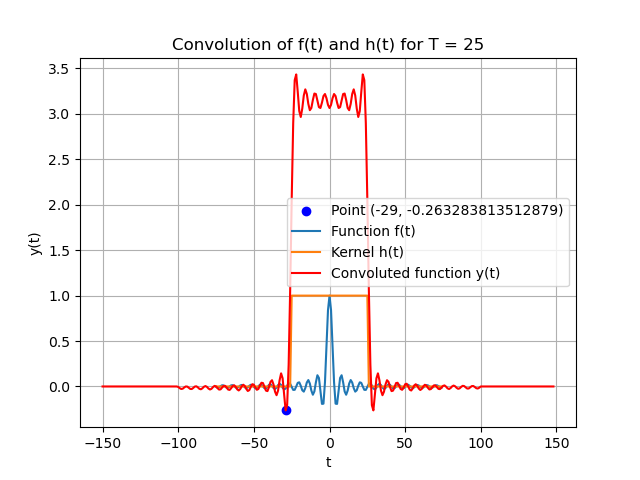
\includegraphics[width=0.6\textwidth]{figs/Conv_sinc.png}
    \caption{T = 25}
    \label{fig:conv_sinc}
\end{figure}
\newpage
For different values of T, the change in $y(t)$ is depicted in the following - \\
\begin{figure}[h]
    \centering
    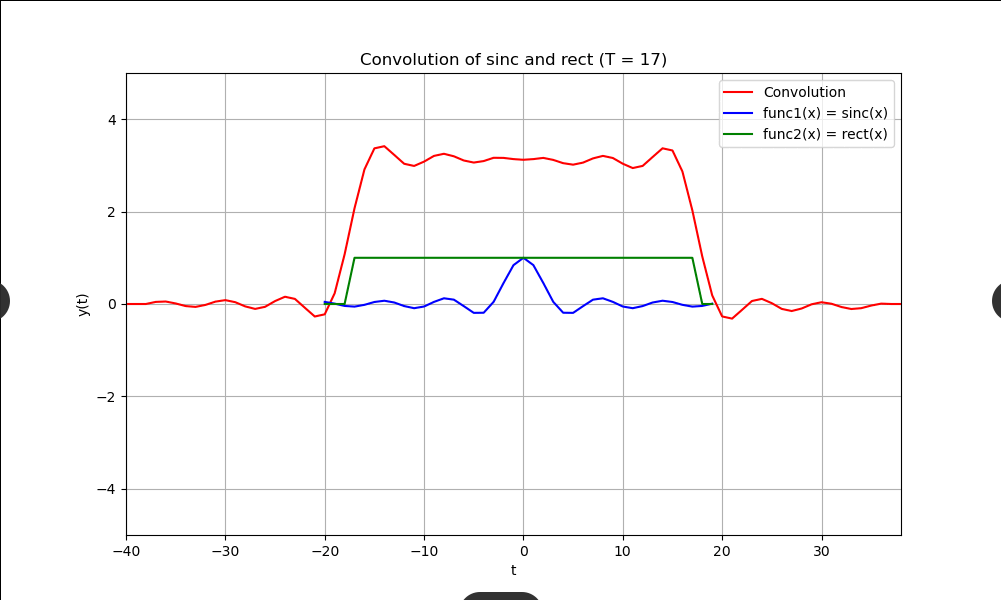
\includegraphics[width=0.6\textwidth]{figs/con1.png}
    \caption{T = 17}
    \label{fig:conv_sinc}
\end{figure}
\begin{figure}[h]
    \centering
    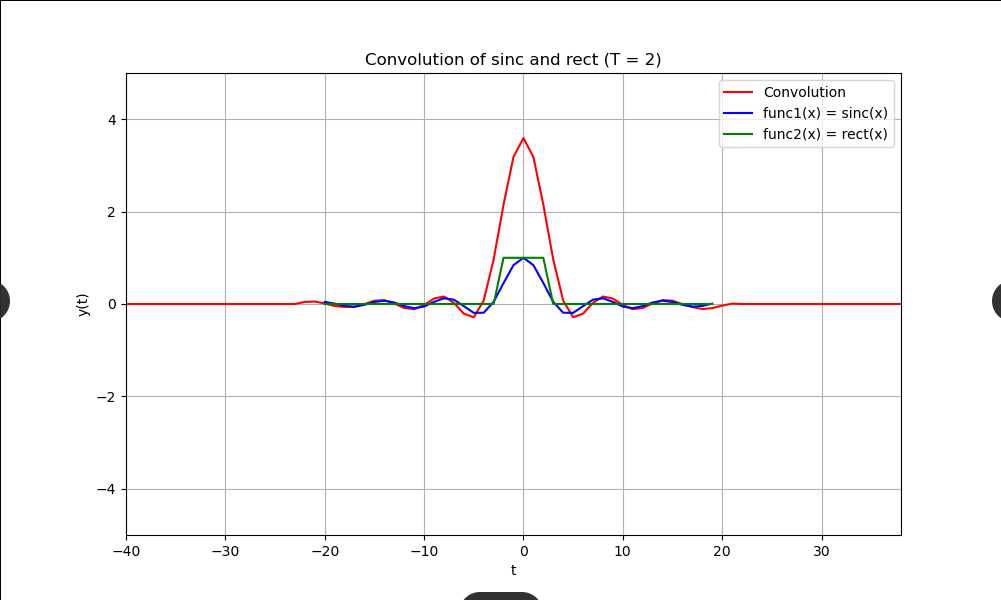
\includegraphics[width=0.6\textwidth]{figs/con2.png}
    \caption{T = 2}
    \label{fig:conv_sinc}
\end{figure}
\begin{figure}[h]
    \centering
    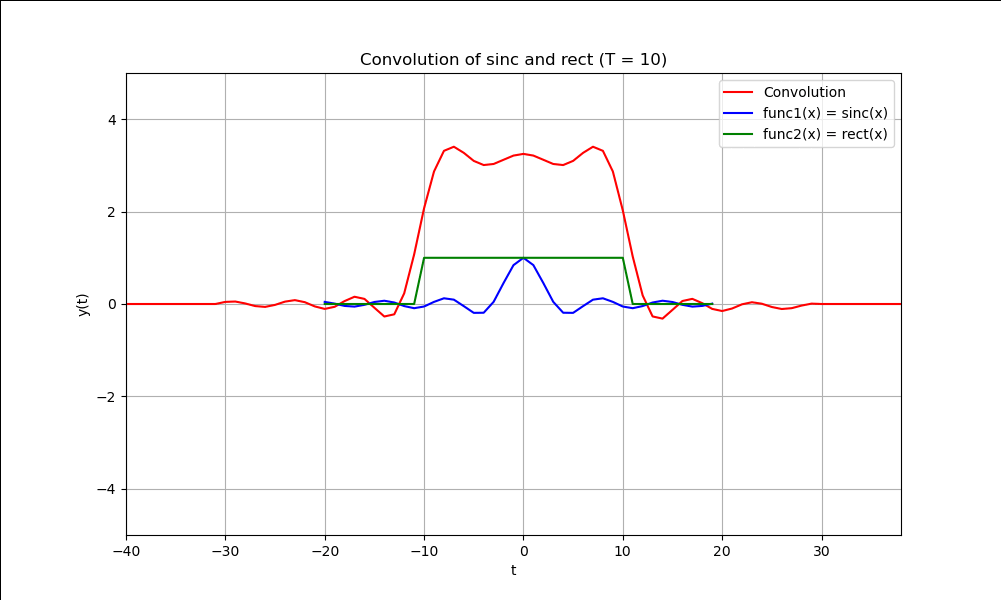
\includegraphics[width=0.6\textwidth]{figs/con3.png}
    \caption{T = 10}
    \label{fig:conv_sinc}
\end{figure}
\begin{figure}[h]
    \centering
    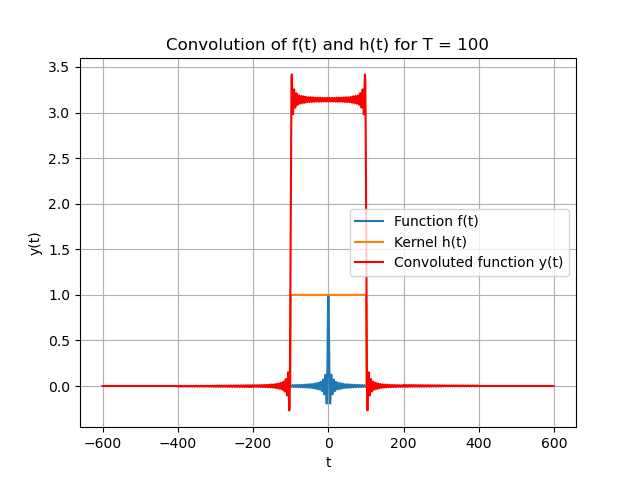
\includegraphics[width=0.6\textwidth]{figs/con4.png}
    \caption{T = 100}
    \label{fig:conv_sinc}
\end{figure}
\begin{figure}[h]
    \centering
    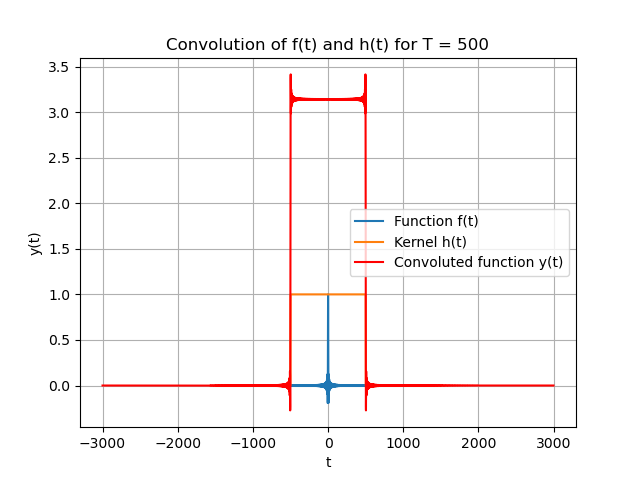
\includegraphics[width=0.6\textwidth]{figs/con5.png}
    \caption{T = 500}
    \label{fig:conv_sinc}
\end{figure}
\newpage
It can be seen that as $T$ increases, $y(t)$ becomes more square.

\newpage
\subsection{Considering the kernel for $t>0$}
The response of the system for different values of $T$ are as follows - \\
\begin{figure}[h]
    \centering
    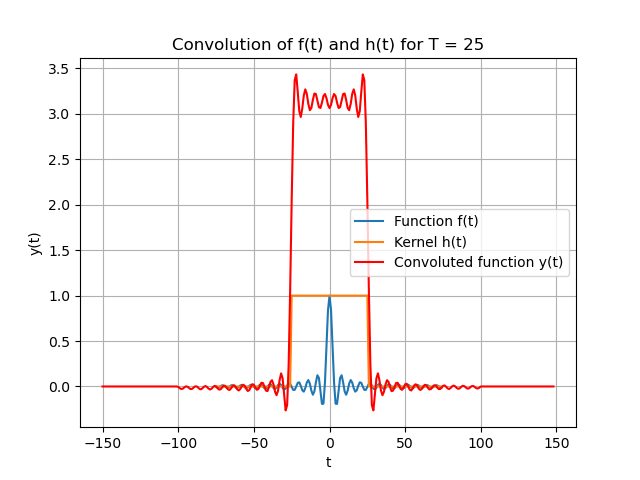
\includegraphics[width=0.6\textwidth]{figs/conv_sinc.png}
    \caption{T = 25}
    \label{fig:conv_sinc}
\end{figure}
\begin{figure}[h]
    \centering
    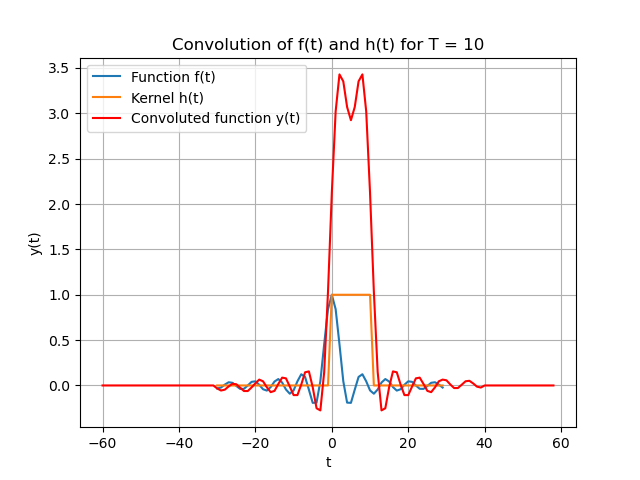
\includegraphics[width=0.6\textwidth]{figs/con6.png}
    \caption{T = 10}
    \label{fig:conv_sinc}
\end{figure}
\begin{figure}[h]
    \centering
    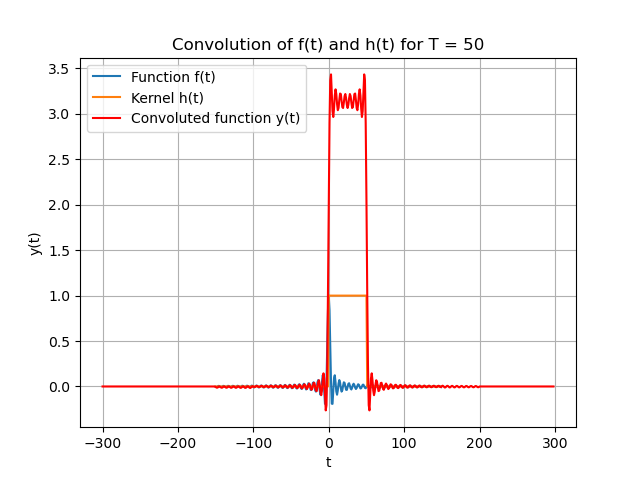
\includegraphics[width=0.6\textwidth]{figs/con7.png}
    \caption{T = 50}
    \label{fig:conv_sinc}
\end{figure}
\begin{figure}[h]
    \centering
    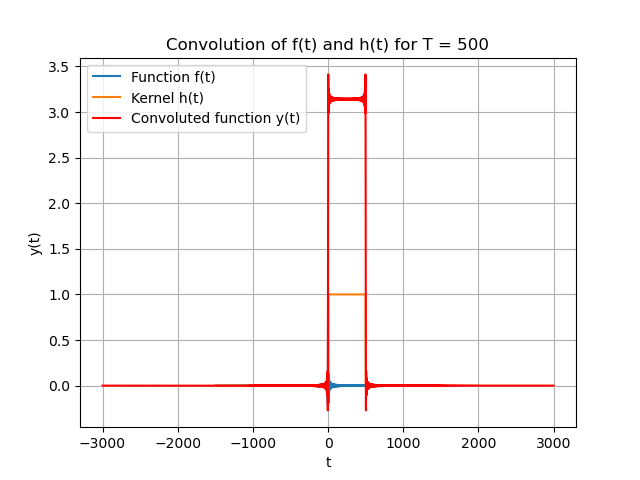
\includegraphics[width=0.6\textwidth]{figs/con8.png}
    \caption{T = 500}
    \label{fig:conv_sinc}
\end{figure}
It can be seen that the width of the convolution becomes half and it becomes shifted to the right.
\newpage

\subsection{Shifting the kernel by $t_{0}$}
Shifting of kernel means moving the kernel to the left or right by an amount, i.e., if the given kernel is shifted by an amount $t_0$, then it becomes, 
\[
h(t) =
\begin{cases}
1, & \text{for } -T \leq t-t_0 \leq T \\
0, & \text{otherwise}
\end{cases}
\]
\[
h(t) =
\begin{cases}
1, & \text{for } -T+t_0 \leq t \leq T+t_0 \\
0, & \text{otherwise}
\end{cases}
\]
If we are convolving a signal with the kernel, at each time $t$, we are sliding the kernel over the signal and computing how much they overlap. So, when we shift the kernel by $t_0$, we are changing when the kernel has its maximum influence.
This can physically mean applying a response $t_0$ time units early (or) $t_0$ time units late depending upon the sign of $t_0$, i.e., if $t_0 > 0$, the response is delayed and is advanced for $t_0 < 0$. This results in the convoluted signal also to be shifted by the same amount, as in figures \ref{fig:rshift} and \ref{fig:lshift} - 
\begin{figure*}[!htb]
    {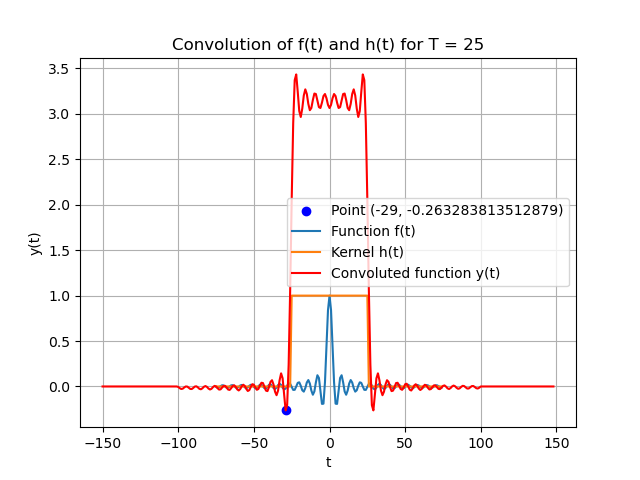
\includegraphics[ width=0.40\textwidth]{figs/Conv_sinc.png}}
    \hspace{\fill}
    {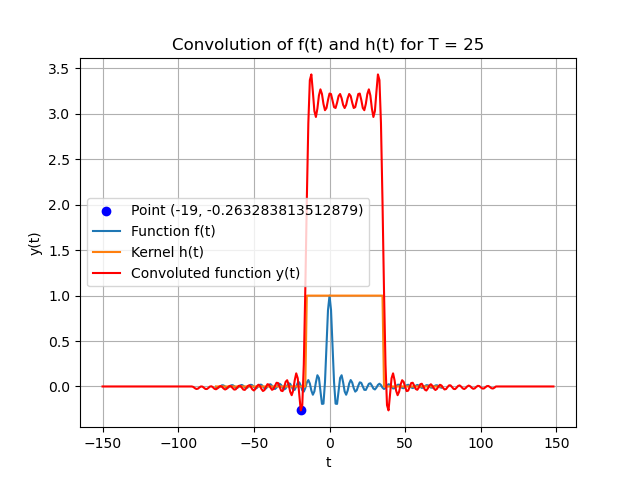
\includegraphics[ width=0.40\textwidth]{figs/conv_shift.png}}
    \hspace{\fill}\\
    \caption{Shifting toward right}
    \label{fig:rshift}
\end{figure*}
\begin{figure*}[!htb]
    {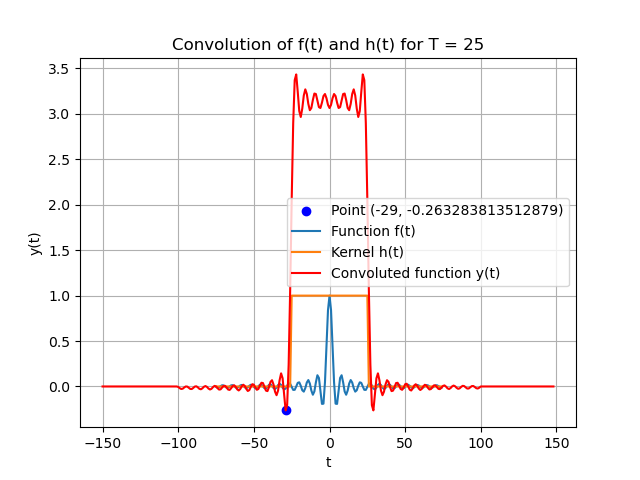
\includegraphics[ width=0.40\textwidth]{figs/Conv_sinc.png}}
    \hspace{\fill}
    {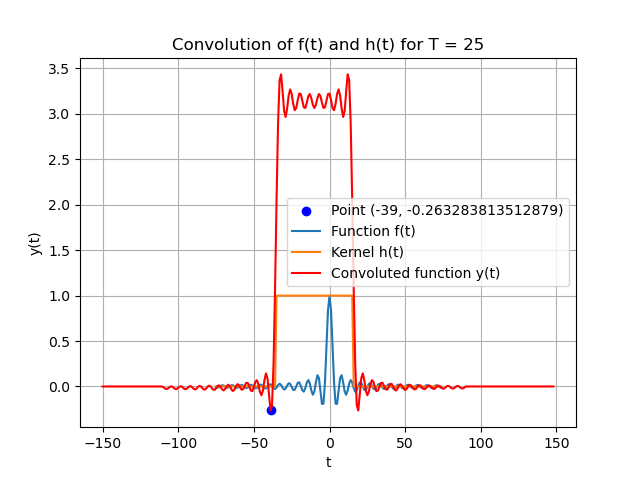
\includegraphics[ width=0.40\textwidth]{figs/conv_left.png}}
    \hspace{\fill}\\
    \caption{Shifting toward left}
    \label{fig:lshift}
\end{figure*}
Shifting of the kernel by 10 units results in shifting of convoluted function by 10 units.
\newpage






	     
